% ========================================
%	Header einbinden
% ========================================

\documentclass[bibtotoc,titlepage]{scrartcl}

% Deutsche Spracheinstellungen
\usepackage[ngerman,german]{babel, varioref}
\usepackage[T1]{fontenc}
\usepackage[utf8]{inputenc}

%\usepackage{marvosym}

\usepackage{amsfonts}
\usepackage{amssymb}
\usepackage{amsmath}
\usepackage{amscd}
\usepackage{amstext}

\usepackage{longtable}

%\usepackage{bibgerm}

\usepackage{footnpag}

\usepackage{ifthen}                 %%% package for conditionals in TeX
\usepackage[amssymb]{SIunits}
%Für textumflossene Bilder und Tablellen
%\usepackage{floatflt} - veraltet

%Für Testzwecke aktivieren, zeigt labels und refs im Text an.
%\usepackage{showkeys}

% Abstand zwischen zwei Absätzen nach DIN (1,5 Zeilen)
% \setlength{\parskip}{1.5ex plus0.5ex minus0.5ex}

% Einrückung am Anfang eines neuen Absatzes nach DIN (keine)
%\setlength{\parindent}{0pt}

% Ränder definieren
% \setlength{\oddsidemargin}{0.3cm}
% \setlength{\textwidth}{15.6cm}

% bessere Bildunterschriften
%\usepackage[center]{caption2}


% Problemlösungen beim Umgang mit Gleitumgebungen
\usepackage{float}

% Nummeriert bis zur Strukturstufe 3 (also <section>, <subsection> und <subsubsection>)
%\setcounter{secnumdepth}{3}

% Führt das Inhaltsverzeichnis bis zur Strukturstufe 3
%\setcounter{tocdepth}{3}
\usepackage[version=3]{mhchem}
	\mhchemoptions{minus-sidebearing-left=0.06em, minus-sidebearing-right=0.11em}
\usepackage{exscale}

\newenvironment{dsm} {\begin{displaymath}} {\end{displaymath}}
\newenvironment{vars} {\begin{center}\scriptsize} {\normalsize \end{center}}


\newcommand {\en} {\varepsilon_0}               % Epsilon-Null aus der Elektrodynamik
\newcommand {\lap} {\; \mathbf{\Delta}}         % Laplace-Operator
\newcommand {\R} { \mathbb{R} }                 % Menge der reellen Zahlen
\newcommand {\e} { \ \mathbf{e} }               % Eulersche Zahl
\renewcommand {\i} { \mathbf{i} }               % komplexe Zahl i
\newcommand {\N} { \mathbb{N} }                 % Menge der nat. Zahlen
\newcommand {\C} { \mathbb{C} }                 % Menge der kompl. Zahlen
\newcommand {\Z} { \mathbb{Z} }                 % Menge der kompl. Zahlen
\newcommand {\limi}[1]{\lim_{#1 \rightarrow \infty}} % Limes unendlich
\newcommand {\sumi}[1]{\sum_{#1=0}^\infty}
\newcommand {\rot} {\; \mathrm{rot} \,}         % Rotation
\newcommand {\grad} {\; \mathrm{grad} \,}       % Gradient
\newcommand {\dive} {\; \mathrm{div} \,}        % Divergenz
\newcommand {\dx} {\; \mathrm{d} }              % Differential d
\newcommand {\cotanh} {\; \mathrm{cotanh} \,}   %Cotangenshyperbolicus
\newcommand {\asinh} {\; \mathrm{areasinh} \,}  %Area-Sinus-Hyp.
\newcommand {\acosh} {\; \mathrm{areacosh} \,}  %Area-Cosinus-H.
\newcommand {\atanh} {\; \mathrm{areatanh} \,}  %Area Tangens-H.
\newcommand {\acoth} {\; \mathrm{areacoth} \,}  % Area-cotangens
\newcommand {\Sp} {\; \mathrm{Sp} \,}
\newcommand {\mbe} {\stackrel{\text{!}}{=}}     %Must Be Equal
\newcommand{\qed} { \hfill $\square$\\}
\renewcommand{\i} {\imath}
\def\captionsngerman{\def\figurename{\textbf{Abb.}}}

%%%%%%%%%%%%%%%%%%%%%%%%%%%%%%%%%%%%%%%%%%%%%%%%%%%%%%%%%%%%%%%%%%%%%%%%%%%%
% SWITCH FOR PDFLATEX or LATEX
%%%%%%%%%%%%%%%%%%%%%%%%%%%%%%%%%%%%%%%%%%%%%%%%%%%%%%%%%%%%%%%%%%%%%%%%%%%%
%%%
\ifx\pdfoutput\undefined %%%%%%%%%%%%%%%%%%%%%%%%%%%%%%%%%%%%%%%%% LATEX %%%
%%%
\usepackage[dvips]{graphicx}       %%% graphics for dvips
\DeclareGraphicsExtensions{.eps,.ps}   %%% standard extension for included graphics
\usepackage[ps2pdf]{thumbpdf}      %%% thumbnails for ps2pdf
\usepackage[ps2pdf,                %%% hyper-references for ps2pdf
bookmarks=true,%                   %%% generate bookmarks ...
bookmarksnumbered=true,%           %%% ... with numbers
hypertexnames=false,%              %%% needed for correct links to figures !!!
breaklinks=true,%                  %%% breaks lines, but links are very small
linkbordercolor={0 0 1},%          %%% blue frames around links
pdfborder={0 0 112.0}]{hyperref}%  %%% border-width of frames
%                                      will be multiplied with 0.009 by ps2pdf
%
\hypersetup{ pdfauthor   = {Hannes Franke; Julius Tilly},
pdftitle    = {V301 Innenwiderstand und Leistungsanpassung}, pdfsubject  = {Protokoll FP}, pdfkeywords = {V301, Innenwiderstand, Leistungsanpassung},
pdfcreator  = {LaTeX with hyperref package}, pdfproducer = {dvips
+ ps2pdf} }
%%%
\else %%%%%%%%%%%%%%%%%%%%%%%%%%%%%%%%%%%%%%%%%%%%%%%%%%%%%%%%%% PDFLATEX %%%
%%%
\usepackage[pdftex]{graphicx}      %%% graphics for pdfLaTeX
\DeclareGraphicsExtensions{.pdf}   %%% standard extension for included graphics
\usepackage[pdftex]{thumbpdf}      %%% thumbnails for pdflatex
\usepackage[pdftex,                %%% hyper-references for pdflatex
bookmarks=true,%                   %%% generate bookmarks ...
bookmarksnumbered=true,%           %%% ... with numbers
hypertexnames=false,%              %%% needed for correct links to figures !!!
breaklinks=true,%                  %%% break links if exceeding a single line
linkbordercolor={0 0 1},
linktocpage]{hyperref} %%% blue frames around links
%                                  %%% pdfborder={0 0 1} is the default
\hypersetup{
pdftitle    = {V301 Innenwiderstand und Leistungsanpassung}, 
pdfsubject  = {Protokoll AP}, 
pdfkeywords = {V301, Innenwiderstand, Leistungsanpassung},
pdfsubject  = {Protokoll AP},
pdfkeywords = {V301, Innenwiderstand, Leistungsanpassung}}
%                                  %%% pdfcreator, pdfproducer,
%                                      and CreationDate are automatically set
%                                      by pdflatex !!!
\pdfadjustspacing=1                %%% force LaTeX-like character spacing
\usepackage{epstopdf}
%
\fi %%%%%%%%%%%%%%%%%%%%%%%%%%%%%%%%%%%%%%%%%%%%%%%%%%% END OF CONDITION %%%
%%%%%%%%%%%%%%%%%%%%%%%%%%%%%%%%%%%%%%%%%%%%%%%%%%%%%%%%%%%%%%%%%%%%%%%%%%%%
% seitliche Tabellen und Abbildungen
%\usepackage{rotating}
\usepackage{ae}
\usepackage{
  array,
  booktabs,
  dcolumn
}
\makeatletter 
  \renewenvironment{figure}[1][] {% 
    \ifthenelse{\equal{#1}{}}{% 
      \@float{figure} 
    }{% 
      \@float{figure}[#1]% 
    }% 
    \centering 
  }{% 
    \end@float 
  } 
  \makeatother 


  \makeatletter 
  \renewenvironment{table}[1][] {% 
    \ifthenelse{\equal{#1}{}}{% 
      \@float{table} 
    }{% 
      \@float{table}[#1]% 
    }% 
    \centering 
  }{% 
    \end@float 
  } 
  \makeatother 
%\usepackage{listings}
%\lstloadlanguages{[Visual]Basic}
%\allowdisplaybreaks[1]
%\usepackage{hycap}
%\usepackage{fancyunits}


% ========================================
%	Angaben für das Titelblatt
% ========================================

\title{Versuch 101 - Das Trägheitsmoment\\				% Titel des Versuchs 
\large TU Dortmund, Fakultät Physik\\ 
\normalsize Anfänger-Praktikum}

\author{Jan Adam\\			% Name Praktikumspartner A
{\small \href{jan.adam@tu-dortmund.de}{jan.adam@tu-dortmund.de}}	% Erzeugt interaktiven einen Link
\and						% um einen weiteren Author hinzuzfügen
Dimitrios Skodras\\					% Name Praktikumspartner B
{\small \href{dimitrios.skodras@tu-dortmund.de}{dimitrios.skodras@tu-dortmund.de}}		% Erzeugt interaktiven einen Link
}
\date{30.April 2013}				% Das Datum der Versuchsdurchführung

% ========================================
%	Das Dokument beginnt
% ========================================

\begin{document}

% ========================================
%	Titelblatt erzeugen
% ========================================

\maketitle					% Jetzt wird die Titelseite erzeugt
\thispagestyle{empty} 				% Weder Kopfzeile noch Fußzeile

% ========================================
%	Der Vorspann
% ========================================

%\newpage					% Wenn Verzeichnisse auf einer neuen Seite beginnen sollen
%\pagestyle{empty}				% Weder Kopf- noch Fußzeile für Verzeichnisse

\tableofcontents

%\newpage					% eine neue Seite
%\thispagestyle{empty}				% Weder Kopf- noch Fußzeile für Verzeichnisse
%\listoffigures					% Abbildungsverzeichnis

%\newpage					% eine neue Seite
%\thispagestyle{empty}				% Weder Kopf- noch Fußzeile für Verzeichnisse
%\listoftables					% Tabellenverzeichnis
\newpage					% eine neue Seite


% ========================================
%	Kapitel
% ========================================

\section{Einleitung}
Im Zuge dieses Experiments wird das Trägheitsmoment von Körpern, sowie einer Holzpuppe in zwei verschiedenen Positionen bestimmt. 
Weiterhin soll der Satz von Steiner geprüft werden.

\section{Theorie}
Charakteristisch für die Dynamik von Rotationsbewegungen sind die Größen Drehmoment $M$, Trägheitsmoment $I$ und Winkelbeschleunigung
$\dot \omega$. Das Trägheitsmoment einer punktförmigen masse ist durch $I = m\,r^2$ gegeben. Entsprechend bei ausgedehnten Körpern, bei
denen sich die Massenelemente um eine feste Achse drehen, werden die einzelnen Trägheitsmomente aufsummiert
\begin{align}
 I = \sum_i r^2_i\,m_i.
\end{align}
Bei einer kontinuierlichen Massenverteilung gilt allgemein
\begin{align}
 I = \int r^2 \dx m.
\end{align}
$r$ beschreibt hierbei den Abstand des Massepunkts zur Drehachse. Daher ist das Trägheitsmoment einfacher, symmetrischer Körper leicht
bestimmbar, das komplexerer Körper durch Summation einzelner Trägheitsmomente. Sofern die Drehachse aber nicht mit einem betrachteten
Körper übereinstimmt, sondern um eine Strecke $a$ parallel zu ihr verschoben ist, so kann der Satz von Steiner Abhilfe schaffen
\begin{align}
 I = I_s + m \cdot a^2,
\end{align}
wobei $I_s$ das Trägheitsmoment bezüglich der Drehachse durch den Schwerpunkt ist. 

Bei Rotationsbewegungen von Körpern ist das Drehmoment durch $M = \vec{F} \times \vec{r}$ gegeben. Wenn nun ein schwingbarer Körper
durch eine Auslenkung um den Winkel $\varphi$ aus seiner Ruhelage gebracht wird, wirkt eine Feder ein rücktreibendes Drehmoment auf ihn.
Die Schwingungdauer des Körpers $T$ ist durch sein Trägheitsmoment $I$ und die zu bestimmende Winkelrichtgröße $D$ gegeben
\begin{align}
 T = 2\pi \sqrt{\frac{I}{D}}.
 \label{eq_periode}
\end{align}
Das Drehmoment ist mit der Winkelrichtgröße über den Auslenkwinkel verknüpft
\begin{align}
 D = \frac{M}{\varphi}.
 \label{eq_winkel}
\end{align}

\section{Durchführung}
In Abbildung \eqref{pic_aufbau} ist der Aufbau skizziert. Der zu untersuchende Körper ist mit einer Feder gekoppelt, deren Winkelrichtgröße
es zu bestimmen gilt. Wenn man eine Federwaage senkrecht zum Radius der vom Körper beschriebenen Kreisbahn mit einem Haken an der Stange
in einem bestimmten Abstand $r$ ansetzt, misst man für eine Auslenkung $varphi$ eine Kraft $F$. Mit der vorausgesetzten Orthogonalität
des Kraft- und Ortsvektors, kann man die Winkelrichtgröße nach \eqref{eq_winkel} berechnen
\begin{align}
 D = \frac{F\cdot r}{\varphi}.
\end{align}

\begin{figure}[H]
 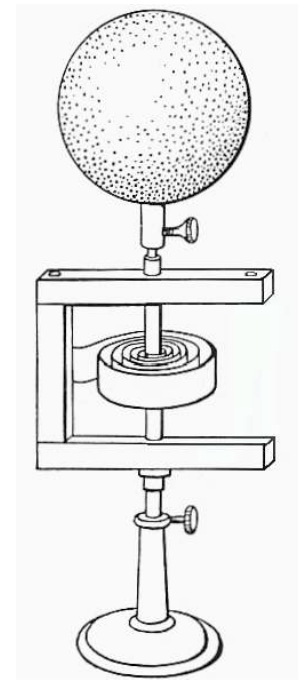
\includegraphics[width=0.3\textwidth]{pics/aufbau.png}
 \caption{Experimenteller Versuchsaufbau (aus Versuchsanleitung)}
 \label{pic_aufbau}
\end{figure}

Selbst ohne Körper hat die Drillachse ein Eigenträgheitsmoment $I_D$, welches über eine massearme Stange mit zwei Gewichten in Abstand $a$
, welche senkrecht zur Achse angebracht, ermittelt werden kann. Das System, in Schwingung gebracht, oszilliert harmonisch mit einer 
zu messenden Periodendauer $T$. Nach \eqref{eq_periode} kann $I_D$ bestimmt werden.

Das Trägheitsmoment zweier verschiedener Zylinder wird ebenfalls durch Messung von Periodendauer, sowie Ausdehnungen und Masse bestimmt.
\eqref{eq_periode} liefert ebenfalls die Lösung.

Für eine Holzpuppe soll das Trägheitsmoment in zwei Stellungen (vergleiche Abbildung \ref{pic_puppe}) berechnet werden. Hierbei werden
die einzelnen Bestandteile als Zylinder angenähert und ihre einzelnen Trägheitsmomente aufsummiert.

\begin{figure}[H]
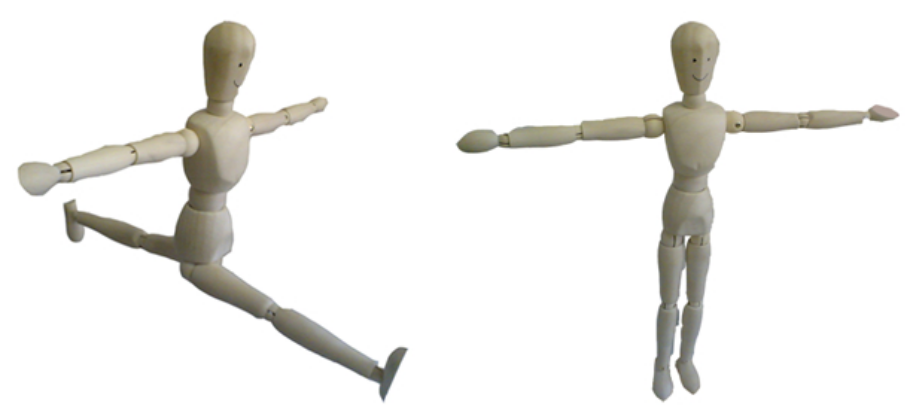
\includegraphics[width=0.8\textwidth]{pics/puppe.png}
\caption{Verwandte Stellungen der Holzpuppe (101 - Trägheitsmomente starrer Körper)}
\label{pic_puppe}
\end{figure}






\section{Auswertung}

\section{Diskussion}

% ========================================
%	Literaturverzeichnis
% ========================================

%\bibliographystyle{plainnat}			% Bibliographie-Style auswählen
%\bibliography{BIBDATEI}			% Literaturverzeichnis

% ========================================
%	Das Dokument endent
% ========================================

\end{document}
